\subsection{Memasukkan Kupon}
Halaman ini hanya dapat diakses oleh pengguna yang sudah terdaftar dan masuk/\textit{login} ke dalam sistem. Pada halaman ini terdapat elemen-elemen halaman \textit{chatting} pada umumnya, yaitu elemen \textit{input} pesan, tombol Kirim, dan riwayat beberapa pesan sebelumnya. Spesifikasi kasus penggunaan dapat dilihat pada Tabel \ref{uc04.05}.\\
\indent Terdapat logika \textit{view} dan alur proses khusus dikarenakan sifat pengiriman dan penerimaan pesan yang realtime, sehingga dibangun diatas Node.js dan menggunakan Socket.io. Masing-masing logika tersebut dapat dijabarkan sebagai berikut:
\begin{enumerate}
	\item Logika \textit{back-end} ditulis menggunakan PHP yang dicantumkan dalam Kode Sumber \ref{cdbe.04-06x}; dan
	\item Logika \textit{view} ditulis menggunakan jQuery yang dicantumkan dalam Kode Sumber \ref{cdjq.04-06x};
\end{enumerate}

\begin{figure}[H]
	\centering
	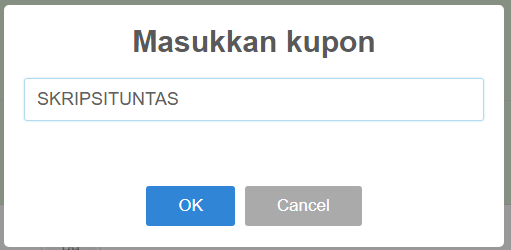
\includegraphics[width=\textwidth]{images/bab4/ui/04-06.png}
	\caption{Halaman Antarmuka Memasukkan Kupon}
	\label{ui.04-06x}
\end{figure}

\begin{lstlisting}[label=cdbe.04-06x,style=php,caption=Kode Sumber \textit{back-end} Memasukkan Kupon]

/** 
* File : app/Http/Controllers/CouponController
* Memproses request ajax
* Method : any
*/

public function submitCoupon(Request $request)
{
	$id_bid = $request['bid'];
	$bid = BidRepository::getBidDetail($id_bid);
	//            edit adding request whether the coupon is expired

	$user = Auth::user();

	$result = $this->couponRepository
	  ->submitCoupon(
	      $user
	      , $bid
	      , $request['coupon']
	  );
	return response()
	    ->json($result);

}

\end{lstlisting}

\begin{lstlisting}[label=cdjq.04-06x,style=htmlcssjs,caption=Kode Sumber \textit{View Logic} Memasukkan Kupon]

/** 
* Menggunakan tools SweetAlert
*/
swal({
 title: 'Masukkan kupon',
 input: 'text',
 showCancelButton: true,
 inputValidator: function (value) {
     return new Promise(function (resolve, reject) {
         if (value) {
             resolve()
         } else {
             reject('Kupon tidak boleh kosong!')
         }
     })
 }
}).then(function (couponName) {
 $.ajax({
   url : "{{ route('coupon.submit') }}",
   type : 'post',
   data: { token : token,
            _token : "{{ csrf_token() }}",
            bid : bid ,
            coupon: "couponName" },
   xhrFields: {
       withCredentials: true
   }
})
   .fail(function (jqXHR, textStatus, errorThrown) {
     return new Promise(function (resolve, reject) {
	       if (value) {
	           resolve()
	       } else {
	           reject(errorThrown)
	       }
     });

   })
   .done(function (result, textStatus, jqXHR) {
       var resp = JSON.parse(result);

       if(resp.status){
         var msgShow;
         if(resp.new_price == -1) msgShow = 'Anda mendapat promo ongkos kirim';
         else if(resp.new_price>0) msgShow = 'Harga barang menjadi ' + result.new_price;
         msgShow = msgShow +  "Anda akan dihubungi admin untuk lebih lanjutnya :)";

         swal(
             'Sukses!',
             msgShow,
             'success'
         );
       }
       else showStatus(resp.msg, false);
   });
})

\end{lstlisting}


